
% Default to the notebook output style

    


% Inherit from the specified cell style.




    
\documentclass[11pt, french]{article}

    
    
    \usepackage[T1]{fontenc}
    \usepackage{babel}
    % Nicer default font (+ math font) than Computer Modern for most use cases
    \usepackage{mathpazo}

    % Basic figure setup, for now with no caption control since it's done
    % automatically by Pandoc (which extracts ![](path) syntax from Markdown).
    \usepackage{graphicx}
    % We will generate all images so they have a width \maxwidth. This means
    % that they will get their normal width if they fit onto the page, but
    % are scaled down if they would overflow the margins.
    \makeatletter
    \def\maxwidth{\ifdim\Gin@nat@width>\linewidth\linewidth
    \else\Gin@nat@width\fi}
    \makeatother
    \let\Oldincludegraphics\includegraphics
    % Set max figure width to be 80% of text width, for now hardcoded.
    \renewcommand{\includegraphics}[1]{\Oldincludegraphics[width=.8\maxwidth]{#1}}
    % Ensure that by default, figures have no caption (until we provide a
    % proper Figure object with a Caption API and a way to capture that
    % in the conversion process - todo).
    \usepackage{caption}
    \DeclareCaptionLabelFormat{nolabel}{}
    \captionsetup{labelformat=nolabel}

    \usepackage{adjustbox} % Used to constrain images to a maximum size 
    \usepackage{xcolor} % Allow colors to be defined
    \usepackage{enumerate} % Needed for markdown enumerations to work
    \usepackage{geometry} % Used to adjust the document margins
    \usepackage{amsmath} % Equations
    \usepackage{amssymb} % Equations
    \usepackage{textcomp} % defines textquotesingle
    % Hack from http://tex.stackexchange.com/a/47451/13684:
    \AtBeginDocument{%
        \def\PYZsq{\textquotesingle}% Upright quotes in Pygmentized code
    }
    \usepackage{upquote} % Upright quotes for verbatim code
    \usepackage{eurosym} % defines \euro
    \usepackage[mathletters]{ucs} % Extended unicode (utf-8) support
    \usepackage[utf8x]{inputenc} % Allow utf-8 characters in the tex document
    \usepackage{fancyvrb} % verbatim replacement that allows latex
    \usepackage{grffile} % extends the file name processing of package graphics 
                         % to support a larger range 
    % The hyperref package gives us a pdf with properly built
    % internal navigation ('pdf bookmarks' for the table of contents,
    % internal cross-reference links, web links for URLs, etc.)
    \usepackage{hyperref}
    \usepackage{longtable} % longtable support required by pandoc >1.10
    \usepackage{booktabs}  % table support for pandoc > 1.12.2
    \usepackage[inline]{enumitem} % IRkernel/repr support (it uses the enumerate* environment)
    \usepackage[normalem]{ulem} % ulem is needed to support strikethroughs (\sout)
                                % normalem makes italics be italics, not underlines
    \usepackage{mathrsfs}
    

    
    
    % Colors for the hyperref package
    \definecolor{urlcolor}{rgb}{0,.145,.698}
    \definecolor{linkcolor}{rgb}{.71,0.21,0.01}
    \definecolor{citecolor}{rgb}{.12,.54,.11}

    % ANSI colors
    \definecolor{ansi-black}{HTML}{3E424D}
    \definecolor{ansi-black-intense}{HTML}{282C36}
    \definecolor{ansi-red}{HTML}{E75C58}
    \definecolor{ansi-red-intense}{HTML}{B22B31}
    \definecolor{ansi-green}{HTML}{00A250}
    \definecolor{ansi-green-intense}{HTML}{007427}
    \definecolor{ansi-yellow}{HTML}{DDB62B}
    \definecolor{ansi-yellow-intense}{HTML}{B27D12}
    \definecolor{ansi-blue}{HTML}{208FFB}
    \definecolor{ansi-blue-intense}{HTML}{0065CA}
    \definecolor{ansi-magenta}{HTML}{D160C4}
    \definecolor{ansi-magenta-intense}{HTML}{A03196}
    \definecolor{ansi-cyan}{HTML}{60C6C8}
    \definecolor{ansi-cyan-intense}{HTML}{258F8F}
    \definecolor{ansi-white}{HTML}{C5C1B4}
    \definecolor{ansi-white-intense}{HTML}{A1A6B2}
    \definecolor{ansi-default-inverse-fg}{HTML}{FFFFFF}
    \definecolor{ansi-default-inverse-bg}{HTML}{000000}

    % commands and environments needed by pandoc snippets
    % extracted from the output of `pandoc -s`
    \providecommand{\tightlist}{%
      \setlength{\itemsep}{0pt}\setlength{\parskip}{0pt}}
    \DefineVerbatimEnvironment{Highlighting}{Verbatim}{commandchars=\\\{\}}
    % Add ',fontsize=\small' for more characters per line
    \newenvironment{Shaded}{}{}
    \newcommand{\KeywordTok}[1]{\textcolor[rgb]{0.00,0.44,0.13}{\textbf{{#1}}}}
    \newcommand{\DataTypeTok}[1]{\textcolor[rgb]{0.56,0.13,0.00}{{#1}}}
    \newcommand{\DecValTok}[1]{\textcolor[rgb]{0.25,0.63,0.44}{{#1}}}
    \newcommand{\BaseNTok}[1]{\textcolor[rgb]{0.25,0.63,0.44}{{#1}}}
    \newcommand{\FloatTok}[1]{\textcolor[rgb]{0.25,0.63,0.44}{{#1}}}
    \newcommand{\CharTok}[1]{\textcolor[rgb]{0.25,0.44,0.63}{{#1}}}
    \newcommand{\StringTok}[1]{\textcolor[rgb]{0.25,0.44,0.63}{{#1}}}
    \newcommand{\CommentTok}[1]{\textcolor[rgb]{0.38,0.63,0.69}{\textit{{#1}}}}
    \newcommand{\OtherTok}[1]{\textcolor[rgb]{0.00,0.44,0.13}{{#1}}}
    \newcommand{\AlertTok}[1]{\textcolor[rgb]{1.00,0.00,0.00}{\textbf{{#1}}}}
    \newcommand{\FunctionTok}[1]{\textcolor[rgb]{0.02,0.16,0.49}{{#1}}}
    \newcommand{\RegionMarkerTok}[1]{{#1}}
    \newcommand{\ErrorTok}[1]{\textcolor[rgb]{1.00,0.00,0.00}{\textbf{{#1}}}}
    \newcommand{\NormalTok}[1]{{#1}}
    
    % Additional commands for more recent versions of Pandoc
    \newcommand{\ConstantTok}[1]{\textcolor[rgb]{0.53,0.00,0.00}{{#1}}}
    \newcommand{\SpecialCharTok}[1]{\textcolor[rgb]{0.25,0.44,0.63}{{#1}}}
    \newcommand{\VerbatimStringTok}[1]{\textcolor[rgb]{0.25,0.44,0.63}{{#1}}}
    \newcommand{\SpecialStringTok}[1]{\textcolor[rgb]{0.73,0.40,0.53}{{#1}}}
    \newcommand{\ImportTok}[1]{{#1}}
    \newcommand{\DocumentationTok}[1]{\textcolor[rgb]{0.73,0.13,0.13}{\textit{{#1}}}}
    \newcommand{\AnnotationTok}[1]{\textcolor[rgb]{0.38,0.63,0.69}{\textbf{\textit{{#1}}}}}
    \newcommand{\CommentVarTok}[1]{\textcolor[rgb]{0.38,0.63,0.69}{\textbf{\textit{{#1}}}}}
    \newcommand{\VariableTok}[1]{\textcolor[rgb]{0.10,0.09,0.49}{{#1}}}
    \newcommand{\ControlFlowTok}[1]{\textcolor[rgb]{0.00,0.44,0.13}{\textbf{{#1}}}}
    \newcommand{\OperatorTok}[1]{\textcolor[rgb]{0.40,0.40,0.40}{{#1}}}
    \newcommand{\BuiltInTok}[1]{{#1}}
    \newcommand{\ExtensionTok}[1]{{#1}}
    \newcommand{\PreprocessorTok}[1]{\textcolor[rgb]{0.74,0.48,0.00}{{#1}}}
    \newcommand{\AttributeTok}[1]{\textcolor[rgb]{0.49,0.56,0.16}{{#1}}}
    \newcommand{\InformationTok}[1]{\textcolor[rgb]{0.38,0.63,0.69}{\textbf{\textit{{#1}}}}}
    \newcommand{\WarningTok}[1]{\textcolor[rgb]{0.38,0.63,0.69}{\textbf{\textit{{#1}}}}}
    
    
    % Define a nice break command that doesn't care if a line doesn't already
    % exist.
    \def\br{\hspace*{\fill} \\* }
    % Math Jax compatibility definitions
    \def\gt{>}
    \def\lt{<}
    \let\Oldtex\TeX
    \let\Oldlatex\LaTeX
    \renewcommand{\TeX}{\textrm{\Oldtex}}
    \renewcommand{\LaTeX}{\textrm{\Oldlatex}}
    % Document parameters
    % Document title
    \title{Chap. III Travailler en base 2, 10 ou 16}
    
    
    
    
    

    % Pygments definitions
    
\makeatletter
\def\PY@reset{\let\PY@it=\relax \let\PY@bf=\relax%
    \let\PY@ul=\relax \let\PY@tc=\relax%
    \let\PY@bc=\relax \let\PY@ff=\relax}
\def\PY@tok#1{\csname PY@tok@#1\endcsname}
\def\PY@toks#1+{\ifx\relax#1\empty\else%
    \PY@tok{#1}\expandafter\PY@toks\fi}
\def\PY@do#1{\PY@bc{\PY@tc{\PY@ul{%
    \PY@it{\PY@bf{\PY@ff{#1}}}}}}}
\def\PY#1#2{\PY@reset\PY@toks#1+\relax+\PY@do{#2}}

\expandafter\def\csname PY@tok@w\endcsname{\def\PY@tc##1{\textcolor[rgb]{0.73,0.73,0.73}{##1}}}
\expandafter\def\csname PY@tok@c\endcsname{\let\PY@it=\textit\def\PY@tc##1{\textcolor[rgb]{0.25,0.50,0.50}{##1}}}
\expandafter\def\csname PY@tok@cp\endcsname{\def\PY@tc##1{\textcolor[rgb]{0.74,0.48,0.00}{##1}}}
\expandafter\def\csname PY@tok@k\endcsname{\let\PY@bf=\textbf\def\PY@tc##1{\textcolor[rgb]{0.00,0.50,0.00}{##1}}}
\expandafter\def\csname PY@tok@kp\endcsname{\def\PY@tc##1{\textcolor[rgb]{0.00,0.50,0.00}{##1}}}
\expandafter\def\csname PY@tok@kt\endcsname{\def\PY@tc##1{\textcolor[rgb]{0.69,0.00,0.25}{##1}}}
\expandafter\def\csname PY@tok@o\endcsname{\def\PY@tc##1{\textcolor[rgb]{0.40,0.40,0.40}{##1}}}
\expandafter\def\csname PY@tok@ow\endcsname{\let\PY@bf=\textbf\def\PY@tc##1{\textcolor[rgb]{0.67,0.13,1.00}{##1}}}
\expandafter\def\csname PY@tok@nb\endcsname{\def\PY@tc##1{\textcolor[rgb]{0.00,0.50,0.00}{##1}}}
\expandafter\def\csname PY@tok@nf\endcsname{\def\PY@tc##1{\textcolor[rgb]{0.00,0.00,1.00}{##1}}}
\expandafter\def\csname PY@tok@nc\endcsname{\let\PY@bf=\textbf\def\PY@tc##1{\textcolor[rgb]{0.00,0.00,1.00}{##1}}}
\expandafter\def\csname PY@tok@nn\endcsname{\let\PY@bf=\textbf\def\PY@tc##1{\textcolor[rgb]{0.00,0.00,1.00}{##1}}}
\expandafter\def\csname PY@tok@ne\endcsname{\let\PY@bf=\textbf\def\PY@tc##1{\textcolor[rgb]{0.82,0.25,0.23}{##1}}}
\expandafter\def\csname PY@tok@nv\endcsname{\def\PY@tc##1{\textcolor[rgb]{0.10,0.09,0.49}{##1}}}
\expandafter\def\csname PY@tok@no\endcsname{\def\PY@tc##1{\textcolor[rgb]{0.53,0.00,0.00}{##1}}}
\expandafter\def\csname PY@tok@nl\endcsname{\def\PY@tc##1{\textcolor[rgb]{0.63,0.63,0.00}{##1}}}
\expandafter\def\csname PY@tok@ni\endcsname{\let\PY@bf=\textbf\def\PY@tc##1{\textcolor[rgb]{0.60,0.60,0.60}{##1}}}
\expandafter\def\csname PY@tok@na\endcsname{\def\PY@tc##1{\textcolor[rgb]{0.49,0.56,0.16}{##1}}}
\expandafter\def\csname PY@tok@nt\endcsname{\let\PY@bf=\textbf\def\PY@tc##1{\textcolor[rgb]{0.00,0.50,0.00}{##1}}}
\expandafter\def\csname PY@tok@nd\endcsname{\def\PY@tc##1{\textcolor[rgb]{0.67,0.13,1.00}{##1}}}
\expandafter\def\csname PY@tok@s\endcsname{\def\PY@tc##1{\textcolor[rgb]{0.73,0.13,0.13}{##1}}}
\expandafter\def\csname PY@tok@sd\endcsname{\let\PY@it=\textit\def\PY@tc##1{\textcolor[rgb]{0.73,0.13,0.13}{##1}}}
\expandafter\def\csname PY@tok@si\endcsname{\let\PY@bf=\textbf\def\PY@tc##1{\textcolor[rgb]{0.73,0.40,0.53}{##1}}}
\expandafter\def\csname PY@tok@se\endcsname{\let\PY@bf=\textbf\def\PY@tc##1{\textcolor[rgb]{0.73,0.40,0.13}{##1}}}
\expandafter\def\csname PY@tok@sr\endcsname{\def\PY@tc##1{\textcolor[rgb]{0.73,0.40,0.53}{##1}}}
\expandafter\def\csname PY@tok@ss\endcsname{\def\PY@tc##1{\textcolor[rgb]{0.10,0.09,0.49}{##1}}}
\expandafter\def\csname PY@tok@sx\endcsname{\def\PY@tc##1{\textcolor[rgb]{0.00,0.50,0.00}{##1}}}
\expandafter\def\csname PY@tok@m\endcsname{\def\PY@tc##1{\textcolor[rgb]{0.40,0.40,0.40}{##1}}}
\expandafter\def\csname PY@tok@gh\endcsname{\let\PY@bf=\textbf\def\PY@tc##1{\textcolor[rgb]{0.00,0.00,0.50}{##1}}}
\expandafter\def\csname PY@tok@gu\endcsname{\let\PY@bf=\textbf\def\PY@tc##1{\textcolor[rgb]{0.50,0.00,0.50}{##1}}}
\expandafter\def\csname PY@tok@gd\endcsname{\def\PY@tc##1{\textcolor[rgb]{0.63,0.00,0.00}{##1}}}
\expandafter\def\csname PY@tok@gi\endcsname{\def\PY@tc##1{\textcolor[rgb]{0.00,0.63,0.00}{##1}}}
\expandafter\def\csname PY@tok@gr\endcsname{\def\PY@tc##1{\textcolor[rgb]{1.00,0.00,0.00}{##1}}}
\expandafter\def\csname PY@tok@ge\endcsname{\let\PY@it=\textit}
\expandafter\def\csname PY@tok@gs\endcsname{\let\PY@bf=\textbf}
\expandafter\def\csname PY@tok@gp\endcsname{\let\PY@bf=\textbf\def\PY@tc##1{\textcolor[rgb]{0.00,0.00,0.50}{##1}}}
\expandafter\def\csname PY@tok@go\endcsname{\def\PY@tc##1{\textcolor[rgb]{0.53,0.53,0.53}{##1}}}
\expandafter\def\csname PY@tok@gt\endcsname{\def\PY@tc##1{\textcolor[rgb]{0.00,0.27,0.87}{##1}}}
\expandafter\def\csname PY@tok@err\endcsname{\def\PY@bc##1{\setlength{\fboxsep}{0pt}\fcolorbox[rgb]{1.00,0.00,0.00}{1,1,1}{\strut ##1}}}
\expandafter\def\csname PY@tok@kc\endcsname{\let\PY@bf=\textbf\def\PY@tc##1{\textcolor[rgb]{0.00,0.50,0.00}{##1}}}
\expandafter\def\csname PY@tok@kd\endcsname{\let\PY@bf=\textbf\def\PY@tc##1{\textcolor[rgb]{0.00,0.50,0.00}{##1}}}
\expandafter\def\csname PY@tok@kn\endcsname{\let\PY@bf=\textbf\def\PY@tc##1{\textcolor[rgb]{0.00,0.50,0.00}{##1}}}
\expandafter\def\csname PY@tok@kr\endcsname{\let\PY@bf=\textbf\def\PY@tc##1{\textcolor[rgb]{0.00,0.50,0.00}{##1}}}
\expandafter\def\csname PY@tok@bp\endcsname{\def\PY@tc##1{\textcolor[rgb]{0.00,0.50,0.00}{##1}}}
\expandafter\def\csname PY@tok@fm\endcsname{\def\PY@tc##1{\textcolor[rgb]{0.00,0.00,1.00}{##1}}}
\expandafter\def\csname PY@tok@vc\endcsname{\def\PY@tc##1{\textcolor[rgb]{0.10,0.09,0.49}{##1}}}
\expandafter\def\csname PY@tok@vg\endcsname{\def\PY@tc##1{\textcolor[rgb]{0.10,0.09,0.49}{##1}}}
\expandafter\def\csname PY@tok@vi\endcsname{\def\PY@tc##1{\textcolor[rgb]{0.10,0.09,0.49}{##1}}}
\expandafter\def\csname PY@tok@vm\endcsname{\def\PY@tc##1{\textcolor[rgb]{0.10,0.09,0.49}{##1}}}
\expandafter\def\csname PY@tok@sa\endcsname{\def\PY@tc##1{\textcolor[rgb]{0.73,0.13,0.13}{##1}}}
\expandafter\def\csname PY@tok@sb\endcsname{\def\PY@tc##1{\textcolor[rgb]{0.73,0.13,0.13}{##1}}}
\expandafter\def\csname PY@tok@sc\endcsname{\def\PY@tc##1{\textcolor[rgb]{0.73,0.13,0.13}{##1}}}
\expandafter\def\csname PY@tok@dl\endcsname{\def\PY@tc##1{\textcolor[rgb]{0.73,0.13,0.13}{##1}}}
\expandafter\def\csname PY@tok@s2\endcsname{\def\PY@tc##1{\textcolor[rgb]{0.73,0.13,0.13}{##1}}}
\expandafter\def\csname PY@tok@sh\endcsname{\def\PY@tc##1{\textcolor[rgb]{0.73,0.13,0.13}{##1}}}
\expandafter\def\csname PY@tok@s1\endcsname{\def\PY@tc##1{\textcolor[rgb]{0.73,0.13,0.13}{##1}}}
\expandafter\def\csname PY@tok@mb\endcsname{\def\PY@tc##1{\textcolor[rgb]{0.40,0.40,0.40}{##1}}}
\expandafter\def\csname PY@tok@mf\endcsname{\def\PY@tc##1{\textcolor[rgb]{0.40,0.40,0.40}{##1}}}
\expandafter\def\csname PY@tok@mh\endcsname{\def\PY@tc##1{\textcolor[rgb]{0.40,0.40,0.40}{##1}}}
\expandafter\def\csname PY@tok@mi\endcsname{\def\PY@tc##1{\textcolor[rgb]{0.40,0.40,0.40}{##1}}}
\expandafter\def\csname PY@tok@il\endcsname{\def\PY@tc##1{\textcolor[rgb]{0.40,0.40,0.40}{##1}}}
\expandafter\def\csname PY@tok@mo\endcsname{\def\PY@tc##1{\textcolor[rgb]{0.40,0.40,0.40}{##1}}}
\expandafter\def\csname PY@tok@ch\endcsname{\let\PY@it=\textit\def\PY@tc##1{\textcolor[rgb]{0.25,0.50,0.50}{##1}}}
\expandafter\def\csname PY@tok@cm\endcsname{\let\PY@it=\textit\def\PY@tc##1{\textcolor[rgb]{0.25,0.50,0.50}{##1}}}
\expandafter\def\csname PY@tok@cpf\endcsname{\let\PY@it=\textit\def\PY@tc##1{\textcolor[rgb]{0.25,0.50,0.50}{##1}}}
\expandafter\def\csname PY@tok@c1\endcsname{\let\PY@it=\textit\def\PY@tc##1{\textcolor[rgb]{0.25,0.50,0.50}{##1}}}
\expandafter\def\csname PY@tok@cs\endcsname{\let\PY@it=\textit\def\PY@tc##1{\textcolor[rgb]{0.25,0.50,0.50}{##1}}}

\def\PYZbs{\char`\\}
\def\PYZus{\char`\_}
\def\PYZob{\char`\{}
\def\PYZcb{\char`\}}
\def\PYZca{\char`\^}
\def\PYZam{\char`\&}
\def\PYZlt{\char`\<}
\def\PYZgt{\char`\>}
\def\PYZsh{\char`\#}
\def\PYZpc{\char`\%}
\def\PYZdl{\char`\$}
\def\PYZhy{\char`\-}
\def\PYZsq{\char`\'}
\def\PYZdq{\char`\"}
\def\PYZti{\char`\~}
% for compatibility with earlier versions
\def\PYZat{@}
\def\PYZlb{[}
\def\PYZrb{]}
\makeatother


    % Exact colors from NB
    \definecolor{incolor}{rgb}{0.0, 0.0, 0.5}
    \definecolor{outcolor}{rgb}{0.545, 0.0, 0.0}



    
    % Prevent overflowing lines due to hard-to-break entities
    \sloppy 
    % Setup hyperref package
    \hypersetup{
      breaklinks=true,  % so long urls are correctly broken across lines
      colorlinks=true,
      urlcolor=urlcolor,
      linkcolor=linkcolor,
      citecolor=citecolor,
      }
    % Slightly bigger margins than the latex defaults
    
    \geometry{verbose,tmargin=1in,bmargin=1in,lmargin=1in,rmargin=1in}
    
    
\author{\textsc{Bruno Darid}}
    \begin{document}
     \renewcommand{\contentsname}{\textsc{Plan}}
    
    \maketitle
    \tableofcontents
    
    \hypertarget{repuxe8res-historiques}{%
\section{Repères historiques}\label{repuxe8res-historiques}}

L'invention du système binaire est souvent attribué à tort au savant
allemand
\href{https://fr.wikipedia.org/wiki/Gottfried_Wilhelm_Leibniz\#Syst\%C3\%A8me_binaire}{Wilhelm
Gottfried Leibniz} (1646-1716). En effet, le mathématicien et astronome
anglais
\href{https://fr.wikipedia.org/wiki/Thomas_Harriot\#Le_math\%C3\%A9maticien}{Thomas
Harriot} (1560-1621) avait déjà travaillé sur les systèmes non
décimaux.\\
Leibniz s'inspire des figures de l'empereur chinois Fuxi (-3000) que
l'on peut considérer comme les premières expressions d'un codage binaire.
\begin{figure}[h]
	\begin{center}
		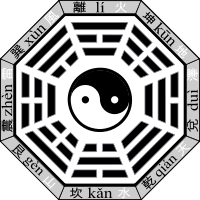
\includegraphics{trigramme_200px.png} 
	\end{center}
	\caption{Fig. \ref{fig:trigramme} -- Trigramme de Fuxi}
	\label{fig:trigramme}
\end{figure}

    \hypertarget{comment-repruxe9senter-des-informations-sur-une-machine-numuxe9rique}{%
\section{Comment représenter des informations sur une machine numérique
?}\label{comment-repruxe9senter-des-informations-sur-une-machine-numuxe9rique}}

    \hypertarget{Unite-d-information}{%
\subsection{Unité d'information}\label{Unite-d-information}}

Les machines numériques sont composées d'éléments manipulant
l'information sous forme de \textbf{deux états distincts}. C'est la
raison pour laquelle on les appelle machine \textbf{binaire}. Par
convention, ces états sont notés \(0\) ou \(1\). En anglais, ces
informations élémentaires sont appelées \emph{binary digit} ou
\textbf{bit}.\\
Un bit permet de représenter \(2^1=2\) informations.\\
\begin{itemize}
\item Citer un système qui nécessite \textbf{un} bit pour coder son
information.\\
\item Combien de bits sont nécessaires pour distinguer les 4 familles d'un
jeu de cartes?
\end{itemize}
En généralisant on a la propriété importante: \(n\) bits permettent de
représenter \(2^n\) informations.
Autres exemples:\\
\begin{itemize}
\item Combien de bits sont nécessaires pour distinguer les 26 lettres de
l'alphabet ?\\
\item Justifier le fait qu'à l'origine 7 bits étaient suffisants pour coder
du texte (\emph{en anglais!})
\end{itemize}
    \begin{Verbatim}[commandchars=\\\{\}]
{\color{incolor}In [{\color{incolor}1}]:} \PY{c+c1}{\PYZsh{}\PYZsh{}\PYZsh{}\PYZsh{}\PYZsh{}\PYZsh{}\PYZsh{}\PYZsh{}\PYZsh{}\PYZsh{}\PYZsh{}\PYZsh{}\PYZsh{}\PYZsh{}\PYZsh{}\PYZsh{}\PYZsh{}\PYZsh{}Réponses aux questions\PYZsh{}\PYZsh{}\PYZsh{}\PYZsh{}\PYZsh{}\PYZsh{}\PYZsh{}\PYZsh{}\PYZsh{}\PYZsh{}\PYZsh{}\PYZsh{}\PYZsh{}\PYZsh{}\PYZsh{}\PYZsh{}\PYZsh{}\PYZsh{}}
        \PY{c+c1}{\PYZsh{} 1) Un détecteur de fumée: présence de fumée activation alarme \PYZhy{}\PYZgt{} état 1}
        \PY{c+c1}{\PYZsh{} pas de fumée, pas d\PYZsq{}alarme \PYZhy{}\PYZgt{} état 0}
        \PY{c+c1}{\PYZsh{} 2) Deux bits sont suffisants (voir schéma)}
\end{Verbatim}

    \begin{Verbatim}[commandchars=\\\{\}]
{\color{incolor}In [{\color{incolor} }]:} \PY{c+c1}{\PYZsh{} 3) 5 bits nécessaire, car 2\PYZca{}4 \PYZlt{} 26 \PYZlt{} 2\PYZca{}5}
        \PY{c+c1}{\PYZsh{} 4) 26*2 (minuscules + majuscules) + 10 (chiffres) + 30(ponctuation) = 92}
        \PY{c+c1}{\PYZsh{} Or 2\PYZca{}6 \PYZlt{} 92 \PYZlt{} 2\PYZca{}7}
\end{Verbatim}

    Les machines numériques manipulent habituellement des groupes de bits.
Ainsi, un groupe de 8 bits forment un \textbf{octet} (!!!! ATTENTION
!!!!! en anglais un \textbf{octet} est traduit par \textbf{BYTE}). Au
delà de 8 bits on utilise le terme \textbf{mot}. On parle par exemple de
mot de 16 bits, de mot de 32 bits (on trouve aussi le terme \emph{double
mot}) ou de mot de 64 bits (ou \emph{quadruple mot}).

    Les quantités d'informations stockées ou manipulées s'expriment avec les
préfixes habituels reliés aux puissances de 10 (1 kilooctet (ko)
\(= 1\times10^3\) octets, 1 mégaoctet (Mo) \(= 1\times10^6\) octets, 1
gigaoctet (Go) \(= 1\times10^9\) octets etc).\\
\emph{Remarque}: certains informaticiens/électroniciens utilisent encore
des définitions de ces quantités exprimées en puissances de 2
(\(2^{10}\), \(2^{20}\), \(2^{30}\), etc). Pour éviter les confusions,
l'International Electrotechnical Commission (IEC) a normalisé ces
appellations en décembre 1998. Voir
\href{https://physics.nist.gov/cuu/Units/binary.html}{lien}.

    \hypertarget{repruxe9sentation-binaire-des-entiers-naturels}{%
\subsection{Représentation binaire des entiers
naturels}\label{repruxe9sentation-binaire-des-entiers-naturels}}

\hypertarget{repruxe9sentation-positionnelle}{%
\subsubsection{Représentation
positionnelle}\label{repruxe9sentation-positionnelle}}

On présente les nombres entiers de manière classique en
\emph{représentation positionnelle}. Par exemple en base 10, la suite
123 signifie \(1\times 10^2+2\times 10^1+3\times 10^0\). En base 2, la
suite 10011 signifie
\(1\times 2^4+0\times 2^3+0\times 2^2+1\times 2^1+1\times 2^0\).\\
Dans un motif binaire, le bit le plus à droite est le \textbf{bit de
poids faible} ou \textbf{LSB} (\emph{Least Significant Bit}). A
l'opposé, le bit le plus à gauche est le \textbf{bit
de poids fort} ou \textbf{MSB} (\emph{Most Significant Bit}). Le bit de
poids faible peut être utilisé pour trouver la parité du nombre: \(0\)
indique un nombre pair et \(1\) un nombre impair.

    \hypertarget{conversion-binaire---duxe9cimal}{%
\subsubsection{Conversion binaire -
décimale}\label{conversion-binaire---duxe9cimal}}

La conversion binaire - décimale d'un entier naturel découle simplement
du mode de représentation positionnelle: on additionne les puissances de
2 présentes dans le motif binaire. Ainsi, pour l'exemple précédent on
a:\\
\(10011_2=(1\times 2^4+0\times 2^3+0\times 2^2+1\times 2^1+1\times 2^0)_{10}=19_{10}\)\\
\emph{Remarque}\\
La base a été indiquée ici en indice, on peut l'omettre lorsqu'il n'y a
pas d'ambiguité.

    \hypertarget{conversion-duxe9cimal---binaire}{%
\subsubsection{Conversion décimale -
binaire}\label{conversion-duxe9cimal---binaire}}

On décompose le nombre entier en une somme de puissance de 2 par
divisions entières successives tant que le quotient est supérieur ou
égal à 2.\\
Exemple: soit \(N=23\) à convertir en binaire

    \begin{Verbatim}[commandchars=\\\{\}]
{\color{incolor}In [{\color{incolor}23}]:} \PY{c}{\PYZpc{}\PYZpc{}latex}
         \PY{k}{\PYZbs{}begin}\PY{n+nb}{\PYZob{}}align*\PY{n+nb}{\PYZcb{}} 
         23 \PY{n+nb}{\PYZam{}}=  2\PY{k}{\PYZbs{}times} 11+1 \PY{k}{\PYZbs{}\PYZbs{}} 
          \PY{n+nb}{\PYZam{}}=  2\PY{k}{\PYZbs{}times}(2\PY{k}{\PYZbs{}times}5 +1)+1\PY{k}{\PYZbs{}\PYZbs{}}
          \PY{n+nb}{\PYZam{}}= 2\PY{k}{\PYZbs{}times}(2\PY{k}{\PYZbs{}times}(2\PY{k}{\PYZbs{}times}2 +1)+1)+1\PY{k}{\PYZbs{}\PYZbs{}}
          \PY{n+nb}{\PYZam{}}= 2\PY{k}{\PYZbs{}times}(2\PY{k}{\PYZbs{}times}(2\PY{k}{\PYZbs{}times}(2\PY{k}{\PYZbs{}times}1+0)+1)+1)+1
         \PY{k}{\PYZbs{}end}\PY{n+nb}{\PYZob{}}align*\PY{n+nb}{\PYZcb{}}
\end{Verbatim}

    \begin{align*} 
23 &=  2\times 11+1 \\ 
 &=  2\times(2\times5 +1)+1\\
 &= 2\times(2\times(2\times2 +1)+1)+1\\
 &= 2\times(2\times(2\times(2\times1+0)+1)+1)+1
\end{align*}

    
    Le résultat est donc \(N=10111_2\). On peut le retrouver en juxtaposant
les restes des divisions \og potences\fg (voir exemple au tableau).\\
Applications
\begin{enumerate}
\item Trouver la représentation binaire de \(77_{10}\) et \(123_{10}\). 
\item Trouver la représentation décimale de \(1101\ 1011_2\).
\end{enumerate}

    \hypertarget{repruxe9sentation-hexaduxe9cimale}{%
\section{Représentation
hexadécimale}\label{repruxe9sentation-hexaduxe9cimale}}

    \hypertarget{Chiffres-hexadecimaux}{%
\subsection{Chiffres hexadécimaux}\label{Chiffres-hexadecimaux}}

La représentation binaire devient rapidement encombrante. On lui préfère
souvent la représentation \emph{hexadécimale} (base 16). L'utilisation
de cette base nécessite 16 caractères. Le tableau ci-dessous présente
ces caractères ainsi que leur équivalence en base 10 et 2.

\begin{figure}[h]
	\begin{center}
		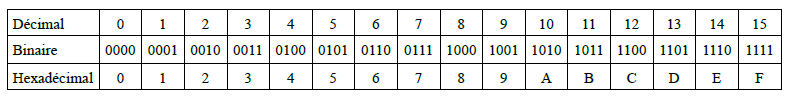
\includegraphics{caracteres_hexa.png} 
	\end{center}
	\caption{Fig. \ref{fig:tabchiffres} -- Valeurs binaire et décimale des chiffres hexadécimaux}
	\label{fig:tabchiffres}
\end{figure}
    \hypertarget{Conversion-decimal-hexa}{%
\subsection{Conversions décimale - hexadécimale}\label{Conversion-decimal-hexa}}
Les principes de conversion décimal-hexdécimal et vice-versa
sont identiques aux principes de conversion vus pour le binaire.\\
Applications 
\begin{enumerate}
\item Trouver la représentation hexdécimale de \(77_{10}\) et
\(123_{10}\). 
\item Trouver la représentation décimale de \(6A0_{16}\).
\end{enumerate}
\hypertarget{conversions-binaire---hexaduxe9cimal}{%
\subsection{Conversions binaire -
hexadécimal}\label{conversions-binaire---hexaduxe9cimal}}

Pour passer du binaire à l'hexadécimal il suffit de grouper les bits par
4 et de les remplacer par leur équivalent hexdécimal (\emph{voir tableau
ci-dessus}).\\
Exemple\\
\(1101\ 1011_2 = DB_{16}\)\\
Pour convertir de l'hexadécimal en binaire, on remplace chaque chiffre
hexadécimal par son équivalent binaire sur 4 bits.\\
Exemple \(7A5_{16}= 0111\ 1010\ 0101_2\)

    \hypertarget{uxe0-retenir}{%
\section{À retenir}\label{uxe0-retenir}}

L'information numérique est manipulée sous forme de \emph{bits}. Les
machines numériques travaillent avec des groupes de bits: des octets (8
bits) ou des mots (16, 32 ou 64 bits).\\
Les nombres entiers sont représentés en machine par des motifs binaires,
c'est-à-dire une décomposition suivant les puissances de 2, obtenue par
divisions successives par 2 par exemple.\\
Afin de limiter l'encombrement des motifs binaires on peut utiliser la
représentation hexadécimale où chaque groupe de 4 bits du nombre binaire
est remplacé par un chiffre hexadécimal compris entre 0 et \(F\). Le
passage du décimal à l'hexadécimal se fait par divisions successives par
16.

    \hypertarget{e1c3-manipulations-binaires-en-python}{%
\section{E1C3 Manipulations binaires en
python}\label{e1c3-manipulations-binaires-en-python}}

\hypertarget{a.-pruxe9ambule-types-natifs}{%
\subsection{Préambule: types
natifs}\label{a.-pruxe9ambule-types-natifs}}

Python possède trois types numériques natifs, parmi lesquels on peux
citer les entiers \textbf{relatifs} (\emph{integers}) et les nombres
décimaux à virgule flottante (\emph{float}). Pour manipuler du texte, on
dispose du type chaine de caractères (\emph{string}). Ces dernières sont
déclarées en étant entourées de double quotes " " ou de simples quotes '
'. Par exemple
\begin{Shaded}
\begin{Highlighting}[]
\NormalTok{mavariable }\OperatorTok{=} \StringTok{"programmation"}
\end{Highlighting}
Pour accéder au type d'un objet \texttt{obj} on utilise la fonction native \texttt{type()} sur cet objet: 
\begin{Highlighting}[]
\StringTok{type(obj)}
\end{Highlighting}
\end{Shaded}

\begin{enumerate}
\item Donner le type des objets suivants: 11, 11.0 et ``11''. 
\item Représentent-ils le même objet ? 
\end{enumerate}

\hypertarget{Convertisseur-dec-binv1}{%
\subsection{Convertisseur decimal binaire version 1}\label{Convertisseur-dec-binv1}}

Python possède une fonction native qui permet la conversion d'un entier
en binaire: la fonction \texttt{bin()}. 
\begin{enumerate}
\item Consulter la documentation associée à cette fonction. 
\item Convertir l'entier 77 en binaire et l'affecter à une variable nommée \texttt{valeurbinaire}. 
\item Quel est le type de \texttt{valeurbinaire} ? 
\item On souhaiterait afficher \texttt{valeurbinaire} sans le préfixe \texttt{0b}. La fonction (on dit
ici \emph{méthode} associée aux chaines de caractères) qui pourrait être
utilisée est \texttt{strip()}. Exemple d'utilisation:

\begin{Shaded}
\begin{Highlighting}[]
\NormalTok{com }\OperatorTok{=} \StringTok{"# Ceci n'est pas un commentaire valide en python"}
\BuiltInTok{print}\NormalTok{(com.strip(}\StringTok{"# "}\NormalTok{))}
\StringTok{Ceci n'est pas un commentaire valide en python}
\end{Highlighting}
\end{Shaded}

\begin{itemize}
\tightlist
\item
  Consulter la documentation associée à \texttt{str.strip}.
\item
  Afficher \texttt{valeurbinaire} sans le préfixe \texttt{0b}.
\end{itemize}
\end{enumerate}
\hypertarget{c.-convertisseur-decimal-binaire-version-2}{%
\subsection{Convertisseur decimal binaire version
2}\label{c.-convertisseur-decimal-binaire-version-2}}

Dans cette partie on va implémenter en python l'algorithme (\textit{voir Fig. \ref{fig:cnvbinaire}}) évoqué au
paragraphe  \ref{conversion-duxe9cimal---binaire}. L'algorithme est écrit en
pseudo-code, dans lequel l'affectation est notée \(\leftarrow\) et la
chaine de caractères vide "".
\begin{figure}[h]
	\begin{center}
		 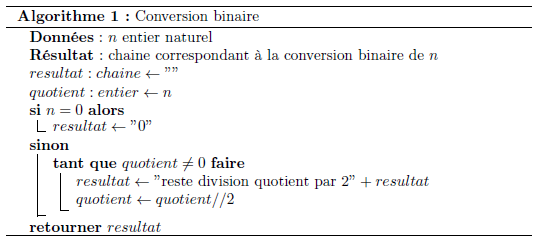
\includegraphics{cnvbinaire.png} 
	\end{center}
	\caption{Fig. \ref{fig:cnvbinaire} -- Algorithme de conversion décimal-binaire}
	\label{fig:cnvbinaire}
\end{figure}

 \begin{enumerate}
 \item Ecrire une fonction en python \texttt{dec2bin(n)} qui retourne la conversion en
binaire d'un entier \(n\).\\
\emph{Indications}: 
	\begin{itemize}
\item en python le reste de la division de \(a\) par \(b\) est obtenu par \texttt{a\ \%\ b}; 
\item la division entière de \(a\) par \(b\) s'obtient par \texttt{a\ //\ b}; 
\item pour convertir un nombre \(x\) en caractère \("x"\) on utilise \texttt{str(x)}.
	\end{itemize}
\item Justifier simplement que la boucle \textbf{Tant que} termine. 
\item \emph{Pour les plus rapides}: retourner le résultat sur 16 bits en complétant le
cas échéant avec des zéros. Indication: se documenter sur la fonction \texttt{str.zfill()}.
\end{enumerate}
    \hypertarget{e2c3-manipulations-hexduxe9cimales-en-python}{%
\section{E2C3 Manipulations hexdécimales en
python}\label{e2c3-manipulations-hexduxe9cimales-en-python}}

\hypertarget{pruxe9ambule}{%
\subsection{Préambule}\label{pruxe9ambule}}

Python possède une fonction native permettant de convertir un entier en
hexadécimal: \texttt{hex()}. 
 \begin{enumerate}
\item Consulter la documentation de \texttt{hex}. 
\item Convertir \(N_1=352_{10}\) en hexadécimal. 
\item Afficher la valeur sans le préfixe `0x'. \emph{Conseil}: voir l'exercice du paragraphe \ref{Convertisseur-dec-binv1}.
\end{enumerate}
\hypertarget{traitement-dune-chaine-hexaduxe9cimale}{%
\subsection{Traitement d'une chaine
hexadécimale}\label{traitement-dune-chaine-hexaduxe9cimale}}

Une fonction dont le code est donnée ci-dessous est proposée.
Malheureusement, une partie de sa spécification n'a pas été complétée.
 \begin{enumerate}
\item Que réalise cette fonction ? Faire des tests avec les nombres
``$10\ FA\ 10\ 00$'' et ``$84\ BD\ 10\ 01$''.
\item Afficher la conversion en entier de ces nombres préalablement transformés par la fonction \texttt{big2little()}.
 \end{enumerate}
 
    \begin{Verbatim}[commandchars=\\\{\}]
{\color{incolor}In [{\color{incolor}3}]:} \PY{k}{def} \PY{n+nf}{big2little}\PY{p}{(}\PY{n}{nh}\PY{p}{)}\PY{p}{:}
            \PY{l+s+sd}{\PYZdq{}\PYZdq{}\PYZdq{}}
        \PY{l+s+sd}{    Retourne .....}
        \PY{l+s+sd}{    On suppose que nh est une chaine de longueur multiple de 2 pouvant}
        \PY{l+s+sd}{    être interprété comme un nombre hexadécimal.}
        \PY{l+s+sd}{    \PYZdq{}\PYZdq{}\PYZdq{}}
            \PY{n}{resultat} \PY{o}{=} \PY{l+s+s2}{\PYZdq{}}\PY{l+s+s2}{\PYZdq{}}
            \PY{n}{l} \PY{o}{=} \PY{n+nb}{len}\PY{p}{(}\PY{n}{nh}\PY{p}{)}
            \PY{k}{for} \PY{n}{i} \PY{o+ow}{in} \PY{n+nb}{range}\PY{p}{(}\PY{l+m+mi}{0}\PY{p}{,}\PY{n}{l}\PY{o}{\PYZhy{}}\PY{l+m+mi}{1}\PY{p}{,}\PY{l+m+mi}{2}\PY{p}{)}\PY{p}{:}
                \PY{n}{resultat} \PY{o}{=} \PY{n}{nh}\PY{p}{[}\PY{n}{i}\PY{p}{:}\PY{n}{i}\PY{o}{+}\PY{l+m+mi}{2}\PY{p}{]} \PY{o}{+} \PY{n}{resultat}
            \PY{k}{return} \PY{n}{resultat}
\end{Verbatim}

    \begin{Verbatim}[commandchars=\\\{\}]
{\color{incolor}In [{\color{incolor}4}]:} \PY{c+c1}{\PYZsh{}\PYZsh{}\PYZsh{}\PYZsh{}\PYZsh{}\PYZsh{}\PYZsh{}\PYZsh{}REPONSES\PYZsh{}\PYZsh{}\PYZsh{}\PYZsh{}\PYZsh{}\PYZsh{}\PYZsh{}\PYZsh{}\PYZsh{}\PYZsh{}}
\end{Verbatim}

    \hypertarget{application-entuxeate-dun-fichier-image}{%
\subsection{Application: entête d'un fichier
image}\label{application-entuxeate-dun-fichier-image}}

Les fichiers images au format
\href{https://fr.wikipedia.org/wiki/Windows_bitmap}{BMP} sont bien
documentés. On peut aisemment consulter les informations avec un éditeur
hexadecimal. Les 2 premiers octets servent à identifier le fichier et
les 4 suivants nous donnent la taille du fichier (\emph{en
hexadécimal!}).\\
En python l'ouverture d'un fichier se fait avec la fonction native
\texttt{open()} et obeit à la construction suivante:

\begin{Shaded}
\begin{Highlighting}[]
\NormalTok{f }\OperatorTok{=} \BuiltInTok{open}\NormalTok{(}\StringTok{'nom_fichier'}\NormalTok{,}\StringTok{'rb'}\NormalTok{)}\CommentTok{#lecture en mode binaire}
\CommentTok{#traitement(s)}
\CommentTok{#}
\NormalTok{f.close()}\CommentTok{#important !!}
\end{Highlighting}
\end{Shaded}

La séquence \texttt{f\ =\ open()} retourne un objet ``fichier'' qui
dispose de nombreuses \emph{méthodes}, parmi lesquelles on peut citer
\texttt{read(n)} qui permet de lire \(n\) octets.\\
\begin{enumerate}
\item Ouvrir le fichier ``alien.bmp'' en lecture binaire. 
\item Lire et afficher le type de fichier. 
\item Lire les 4 octets suivants et les stocker dans une variable \texttt{taille\_big}. 
\item Stocker dans une variable \texttt{taille} la taille du fichier BMP. Il suffit de passer
\texttt{taille\_big} à la fonction \texttt{big2little()}. 
\item Convertir cette taille en entier (fonction \texttt{int()}). Cette valeur est-elle
cohérente avec celle fournie par le système d'exploitation?
\end{enumerate}

    \begin{Verbatim}[commandchars=\\\{\}]
{\color{incolor}In [{\color{incolor} }]:} \PY{c+c1}{\PYZsh{}\PYZsh{}\PYZsh{}\PYZsh{}\PYZsh{}\PYZsh{}\PYZsh{}\PYZsh{}\PYZsh{}\PYZsh{}\PYZsh{}\PYZsh{}\PYZsh{}\PYZsh{}CORRECTION\PYZsh{}\PYZsh{}\PYZsh{}\PYZsh{}\PYZsh{}\PYZsh{}\PYZsh{}\PYZsh{}\PYZsh{}\PYZsh{}\PYZsh{}\PYZsh{}\PYZsh{}\PYZsh{}\PYZsh{}\PYZsh{}\PYZsh{}\PYZsh{}}
        \PY{n}{f} \PY{o}{=} \PY{n+nb}{open}\PY{p}{(}\PY{l+s+s1}{\PYZsq{}}\PY{l+s+s1}{alien.bmp}\PY{l+s+s1}{\PYZsq{}}\PY{p}{,} \PY{l+s+s1}{\PYZsq{}}\PY{l+s+s1}{rb}\PY{l+s+s1}{\PYZsq{}}\PY{p}{)}\PY{c+c1}{\PYZsh{} ouverture du fichier en lecture binaire}
        \PY{n}{type\PYZus{}fichier} \PY{o}{=} \PY{n}{f}\PY{o}{.}\PY{n}{read}\PY{p}{(}\PY{l+m+mi}{2}\PY{p}{)}\PY{c+c1}{\PYZsh{} on lit 2 octets}
        \PY{n+nb}{print}\PY{p}{(}\PY{n}{type\PYZus{}fichier}\PY{p}{)}
        \PY{n}{taille\PYZus{}big} \PY{o}{=} \PY{n}{f}\PY{o}{.}\PY{n}{read}\PY{p}{(}\PY{l+m+mi}{4}\PY{p}{)}\PY{c+c1}{\PYZsh{} on lit les 4 octets suivants}
        \PY{n}{f}\PY{o}{.}\PY{n}{close}\PY{p}{(}\PY{p}{)}\PY{c+c1}{\PYZsh{} on n\PYZsq{}a plus besoin du fichier, on le referme !}
        \PY{n}{taille} \PY{o}{=} \PY{n}{big2little}\PY{p}{(}\PY{n}{taille\PYZus{}big}\PY{p}{)}
        \PY{n+nb}{print}\PY{p}{(}\PY{n+nb}{int}\PY{p}{(}\PY{n}{taille}\PY{p}{,} \PY{l+m+mi}{16}\PY{p}{)}\PY{p}{)}\PY{c+c1}{\PYZsh{} conversion en entier à partir de la base 16}
\end{Verbatim}

    \hypertarget{ruxe9sumuxe9-des-fonctions-python-rencontruxe9es}{%
\section{Résumé des fonctions python
rencontrées}\label{ruxe9sumuxe9-des-fonctions-python-rencontruxe9es}}

Le type d'un objet python \texttt{obj} s'obtient par \texttt{type(obj)}.
Les changements de base se font avec les fonctions
\texttt{int(),\ bin(),\ hex()}. La conversion en chaine de caractères
est réalisée par la fonction \texttt{str()}. Les chaines de caractères
possèdent de nombreuses méthodes. Dans ce chapitre, la méthode
\texttt{strip()} a été utilisée; elle permet d'éliminer des caractères
en début et fin de chaine.\\
La division euclidienne d'un entier \(a\) par un entier \(b\) a
également été abordée: \(a=b\times q + r\). En python, le quotient
s'obtient par \texttt{q\ =\ a\ //\ b} et le reste par
\texttt{r\ =\ a\ \%\ b}.

\vspace{3cm} 
 Ce(tte) œuvre est mise à disposition selon les termes de la Licence
\href{https://creativecommons.org/licenses/by-nc/4.0/}{Creative Commons Attribution - Pas d'Utilisation Commerciale 4.0
International.}
\begin{center}

\includegraphics{Cc-by-nc_icon.svg.png}
\end{center} 
    
    \end{document}
